\section{Spherically constrainted ODE and SDE}

\label{2305:app:spherical_constraint}
\subsection{Spherical constraint for ODE}
Let's recall the update rule for the weights
\begin{equation}
    \w_j^{\i+1} = \frac{\w_j^{\i}-\lr\nabla_{\w_j}\ell(y^{\nu},f_{\Theta^{\nu}}(x^{\nu}))}{\left\lVert\w_j^{\i}-\lr\nabla_{\w_j}\ell(y^{\nu},f_{\Theta^{\nu}}(x^{\nu}))\right\rVert}\sqrt{d},
\end{equation}
we will find the leading order approximation of it and then apply the argument as the unconstrained case for deriving the ODEs.

To shorten the notation we will use \(\loss\) for indicating \(\ell(y^{\nu},f_{\Theta^{\nu}}(x^{\nu}))\).
Let's start by computing the normalization factor
\[\begin{split}
  \frac{1}{\left\|\w^{\nu}_j - \gamma \nabla_{\w_j}{\loss}\right\|} =&
    \left[\left(\w^{\nu}_j - \gamma \nabla_{\w_j}{\loss}\right)\cdot\left(\w^{\nu}_j - \gamma \nabla_{\w_j}{\loss}\right)\right]^{-\frac12} \\
    =&\left[\left\|\w^{\nu}_j\right\|^2 - 2\gamma\w^{\nu}_j\cdot \nabla_{\w_j}{\loss}+\gamma^2\left\|\nabla_{\w_j}{\loss}\right\|^2\right]^{-\frac12} \\
    =&\frac{1}{\sqrt{d}}\left[1- \frac1d\left(2\gamma\w^{\nu}_j\cdot \nabla_{\w_j}{\loss}-\gamma^2\left\|\nabla_{\w_j}{\loss}\right\|^2\right)\right]^{-\frac12} \\
    =&\frac{1}{\sqrt{d}}\left[1+ \frac{1}{2d}\left(2\gamma\w^{\nu}_j\cdot \nabla_{\w_j}{\loss}-\gamma^2\left\|\nabla_{\w_j}{\loss}\right\|^2\right)+\smallo{d^{-1}}\right].
 \end{split}\]
Note that we kept both two terms in the expansion because we can show that both the norm and the scalar product with a weight vector are order 1
\[\begin{split}
  \left\|\nabla_{\w_j}{\loss}\right\|^2 \sim&
    \frac{2\dsp^2\lf^\nu_j}{p^2} \frac{\sum_{i=1}^d \left(x^\nu_i\right)^2}{d}\sim
    \frac{2\dsp^2\lf^\nu_j}{p^2}\frac{\chi^2_d}{d} = \BigO{1},\\
  \w_j\cdot\nabla_{\w_l}{\loss} \sim&
    \frac{2\dsp\lf^\nu_l}{p}\sum_{i=1}^d\frac{w_{j,i}}{\sqrt{d}}\gauss{(0,1)} \sim
    \frac{2\dsp\lf^\nu_l}{p^2}\gauss{\left(0,\sum_{i=1}^d\frac{w^2_{j,i}}{d}\right)} \sim
    \frac{2\dsp\lf^\nu_l}{p^2}\gauss{\left(0,1\right)}= \BigO{1}.
\end{split}\]
We can now plug the expansion back into the original update rule
\[
  \w^{\nu+1}_j =\left(\w^{\nu}_j - \gamma \nabla_{\w_j}{\loss}\right)\left[1+ \frac{1}{2d}\left(2\gamma\w^{\nu}_j\cdot \nabla_{\w_j}{\loss}-\gamma^2\left\|\nabla_{\w_j}{\loss}\right\|^2\right)+\smallo{d^{-1}}\right]\sqrt{d}.
\]
We are ready to go over the steps that take us from the update rule on vector weights
to those on order parameters. We report by way of example the steps performed for \(\M\);
the accounts for \(\Q\) are similar, just a bit more tedious.
\begin{equation}\label{2305:eq:app:m_update_process}
\begin{split}
  \M^{\nu+1}_{j} &= \frac{\w^{\nu+1}_j\cdot\w^*}{d} \\
    &= \left(\M^{\nu}_{j} - \frac{\gamma\w^*\cdot\nabla_{\w_j}{\loss}}{d}\right)\left[1+ \frac{1}{2d}\left(2\gamma\w^{\nu}_j\cdot \nabla_{\w_j}{\loss}-\gamma^2\left\|\nabla_{\w_j}{\loss}\right\|^2\right)+\smallo{d^{-1}}\right]\\
    &= \M^{\nu}_{j} - \frac{\gamma\w^*\cdot\nabla_{\w_j}{\loss}}{d} + \frac{\M^{\nu}_{j}}{2d}\left(2\gamma\w^{\nu}_j\cdot \nabla_{\w_j}{\loss}-\gamma^2\left\|\nabla_{\w_j}{\loss}\right\|^2\right)+\smallo{d^{-1}} \\
    &= \M^{\nu}_{j} +\frac{1}{d}\left[
      \frac{\gamma}{p} \lf_\star\dsp^\nu\lf^\nu_j -
      \frac{\M^{\nu}_{j}}{2}\left(2\frac{\gamma}{p}\dsp^\nu\lf^\nu_j\lf^\nu_j + \frac{\gamma^2}{p^2} {\dsp^\nu\lf^\nu_j}^2\right)
    \right] + \smallo{d^{-1}}.
\end{split}
\end{equation}
% TODO: adjust this part here because probably the Theorem does not hold even in the unconstrainted case...
We can now take the limit \(d\to+\infty\), claiming that the theorem~\cite{veiga2022phase,goldt2019dynamics} proving ODE convergence is still valid. Indeed, the error term $o(d^{-1})$ in Equation~\eqref{2305:eq:app:m_update_process} has an average order of $O(d^{-2})$, which can be absorbed in the term $\Gamma^\nu$ of Theorem A.1 in \cite{veiga2022phase}. The rest of the proof proceeds the same way, noting that the square function can be assumed to be Lipschitz since the dynamics take place on the sphere.

The differential equation that describes the evolution of \(\M\) is
\[
  \dod{\bar\M_j{\left(t\right)}}{t} =\mathbb E_{\vec{\lf},\vec{\lf^* \sim \gauss{(0,\vec{\Omega}{(t)})}}}{\left[ 2\dsp\lf_j \lf_\star - \frac{\bar\M_j{\left(t\right)}}{2}\left(4\dsp\lf_j\lf_j + 4\frac{\gamma}{p} {\dsp}^2\lf_j^2\right)\right]};
\]
Using the definitions introduced in Equations~\eqref{2305:eq:overlapping_spherical_ODE} we can write the equation in a nicer form
\begin{equation} \label{2305:eq:genericsphericalM}
  \dod{\bar\M_j{\left(t\right)}}{t} = \Psi_{j}{(\vec{\Omega})} - \frac{\bar\M_j{\left(t\right)}}{2}\Phi_{jj}{(\vec{\Omega})}.
\end{equation}
Essentially, the spherical constraint can be imposed by using a term proportional to the unconstrained \(\Q\) update.

Without reporting all the calculations, we can write an analogous differential equation for \(\Q\) evolution
\begin{equation} \label{2305:eq:genericsphericalQ}
  \dod{\bar\Q_{jl}{\left(t\right)}}{t} = \Phi_{jl}{(\vec{\Omega})} - \frac{\bar\Q_{jl}{\left(t\right)}}{2}\left(\Phi_{jj}{(\vec{\Omega})}+\Phi_{ll}{(\vec{\Omega})}\right).
\end{equation}
Note that \(\dod{\bar\Q_{jj}{\left(t\right)}}{t}=0\) if \(\Q_{jj}{\left(t\right)}=1\),
as it should be since the norm of spherical vectors must not change.

\begin{figure}
    \centering
    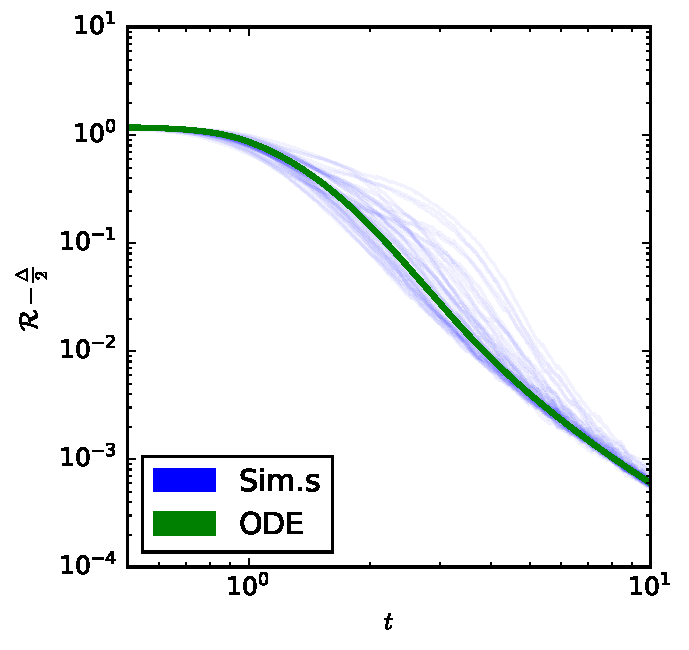
\includegraphics[width=0.49\textwidth]{figs/ode_example-p5}
    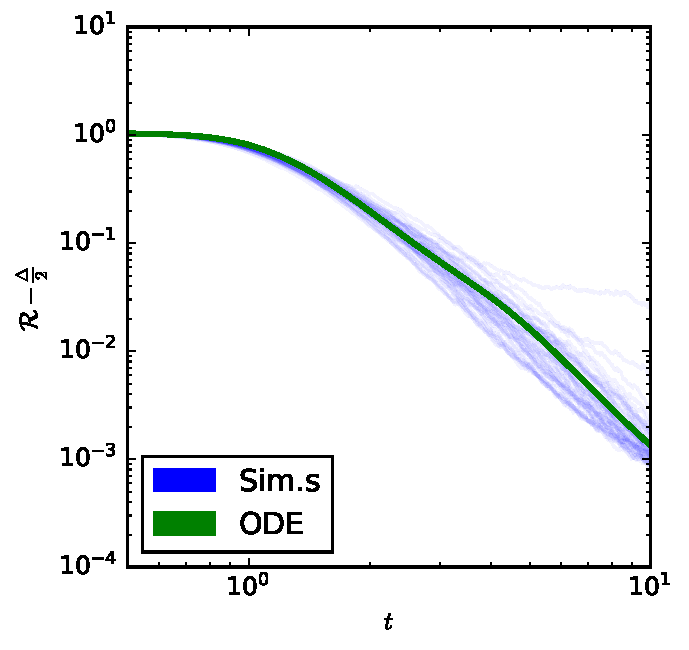
\includegraphics[width=0.49\textwidth]{figs/ode_example-p20}
    \caption{comparison of ODE integration and many SGD runs for \(p=5\) (left) and \(p=20\) (right).
            Both the experiments have \(d=5000\).}
    \label{2305:fig:ODE_prove}
\end{figure}
In Figure~\ref{2305:fig:ODE_prove} we show two examples of integration of ODEs, for different values of \(p\).
Simulating for large but finite \(d\) does not kills the stochasticity in the SGD runs, but we can clearly see how the ODE well describe the dynamics on average.

\subsection{Spherical constraint for SDE}
This subsection we derive the spherical constraint for the SDE, with \(p=1\). We assume that the stochastic process is given
\begin{equation} \label{2305:eq:app:sde_p1}
    \begin{split}
    \dif \M &= \Psi_{1}{(\Omega)}\dif t + \sqrt{\frac{\gamma}{d}}   \vec{\sigma}_\M{(\Omega)} \cdot \dif \b_t \\
    \dif \Q &= \Phi_{11}{(\Omega)}\dif t + \sqrt{\frac{\gamma}{d}}   \vec{\sigma}_\Q{(\Omega)} \cdot \dif \b_t,
    \end{split}
\end{equation}
without providing explicit expressions for \(\vec{\sigma}_\M{(\Omega)}\) and \(\vec{\sigma}_\Q{(\Omega)}\); see Appendix~\ref{2305:app:SDE_with_generic_width} for that.

The derivation is basically following the steps of the previous Section.
Starting from the unconstrainted update rule for the weights
\[
    \w^{\nu+1}_j=\w^{\nu}_j - \gamma \nabla_{\w_j}{\loss},
\]
we can find an expression for the two unconstrained differentials
\begin{equation}\begin{split}
  \dif q &= \frac{-2\gamma \w\cdot\nabla{\loss} + \gamma^2\left\|\nabla{\loss}\right\|^2}{d} \\
  \dif m &= \frac{-\gamma \w_\star\cdot\nabla\loss}{d}.
\end{split}\end{equation}
Since we are forcing the weight on the sphere, the update rule that actually has to be used is
\[
  \w^{\nu+1}_j =\frac{\w^{\nu}_j - \gamma \nabla_{\w_j}{\loss}}{\left\lVert \w^{\nu}_j - \gamma \nabla_{\w_j}{\loss} \right\rVert}\sqrt{d};
\]
multiplying both sides by \(\w_\star\) and subtracting \(m\) we get
\[
  \dif m_S = \frac{m +\dif m}{\left\|\w - \gamma \nabla{\loss}\right\|}\sqrt{d} - m,
\]
where we introduce \(m_S\) to differentiate the constrained variable from \(m\).
Let's estimate the normalization factor
\[
  \begin{split}
  \left\|\w - \gamma \nabla{\loss}\right\| =& \sqrt{(\w - \gamma \nabla{\loss})^2}
                                           =  \sqrt{\w^2 - 2\w\cdot\gamma \nabla{\loss}+\gamma^2\left\|\nabla{\loss}\right\|^2} \\
                                           =& \sqrt{d}\sqrt{\frac{\w^2}{d} + \frac{- 2\w\cdot\gamma \nabla{\loss}+\gamma^2\left\|\nabla{\loss}\right\|^2}{d}}
                                           = \sqrt{d}\sqrt{q +\dif q} \\
                                           =& \sqrt{d}\sqrt{1 +\dif q},
  \end{split}
\]
where in the last step we used the constraint \(q=1\). We can now plug it back in \(\dif m_S\)
\[
  \dif m_S = \frac{m +\dif m}{\sqrt{1 +\dif q}} - m,
\]
and expanding up to leading orders we get
\[\begin{split}
  \dif m_S =& (m +\dif m)(1 +\dif q)^{-\frac12} - m = (m +\dif m)\left(1 -\frac12\dif q + \frac38\dif q^2\right)-m \\
           =& \dif m - \frac{m}{2}\dif q -\frac12 \dif m \dif q + \frac38 m \dif q^2
\end{split}\]
In principle, we can now use the Itô Lemma on differentials Equations~\eqref{2305:eq:app:sde_p1},
obtaining 
\[
  \dif m^2 =    \frac{\gamma}{d}\vec{\sigma}_\M^2{(\Omega)}\dif t, \quad
  \dif q^2 =    \frac{\gamma}{d}\vec{\sigma}^2_\Q{(\Omega)}\dif t, \quad\text{and}\quad
  \dif m \dif q = \frac{\gamma}{d}\vec{\sigma}_\M{(\Omega)} \cdot       \vec{\sigma}_\Q{(\Omega)} \dif t.
\]
It's interesting to note that these lead to a drift correction (and not just stochastic), but it's of second order. As expected, in numerical simulations we can't see the effect for these corrections, hence we neglet them in what follows.
Finally, we write the explicit Brownian motion for the constrained dynamic
\begin{equation} \label{2305:eq:constrained_brownian_motion_p1}
  \dif m_S = \left(\Psi_{1}{(\Omega)} - \frac{m_S}{2}\Phi_{11}{(\Omega)}\right)\dif t
            + \sqrt{\frac{\gamma}{d}}\left(\vec{\sigma}_\M{(\Omega)}-\frac{m_S}{2}\vec{\sigma}_\Q{(\Omega)}\right)\cdot \dif \b_t.
\end{equation}
Of course, all functions depending on \(\Omega\) should be evaluated at \(m=m_S, q=1\).

% %%%%%%%%%%%%%%%%%%%%%%%%%%%%%%%%%%%%%%%%%%%%%%%%%%%%%%%%%%%%%%%%%%%%%%%%%%%%%%%
